% Created 2015-04-22 Wed 23:29
\documentclass[big]{beamer}
\usepackage[utf8]{inputenc}
\usepackage[T1]{fontenc}
\usepackage{fixltx2e}
\usepackage{graphicx}
\usepackage{longtable}
\usepackage{float}
\usepackage{wrapfig}
\usepackage{rotating}
\usepackage[normalem]{ulem}
\usepackage{amsmath}
\usepackage{textcomp}
\usepackage{marvosym}
\usepackage{wasysym}
\usepackage{amssymb}
\usepackage{hyperref}
\tolerance=1000
\usepackage{lmodern}
\usetheme{Boadilla}
\usecolortheme{whale}
\setbeamertemplate{footline}{}
\setbeamertemplate{navigation symbols}{}
\setbeamertemplate{itemize items}[circle]
\setbeamertemplate{enumerate items}[circle]
\setbeamertemplate{alert}{\textbf}
\setbeamertemplate{footline}[frame number]
\usetheme{default}
\author{}
\date{2015-04-23}
\title{Introduction to code profiling in Python}
\hypersetup{
  pdfkeywords={},
  pdfsubject={},
  pdfcreator={Emacs 24.3.50.1 (Org mode 8.2.3a)}}
\begin{document}

\maketitle

\section{Code profiling}
\label{sec-1}

\begin{frame}[label=sec-1-1]{About efficiency}
\begin{block}{Guidelines when programming}
\begin{itemize}
\item 1st: code should be \alert{correct}
\item 2nd: code should be \alert{readable}
\item 3rd: code should be \alert{fast (enough)}
\end{itemize}
\end{block}
\begin{block}{}
\begin{itemize}
\item Priorities might varies from one programmer to another\ldots{}
\item \url{https://xkcd.com/323/}
\end{itemize}
\end{block}
\end{frame}
\begin{frame}[label=sec-1-2]{About efficiency}
\begin{columns}
\begin{column}{0.7\textwidth}
\begin{block}{Donald Knuth}
\begin{quote}
[\ldots{}] premature optimization is the root of all evil (or at least most of it)
\end{quote}
\end{block}
\end{column}
\begin{column}{0.3\textwidth}
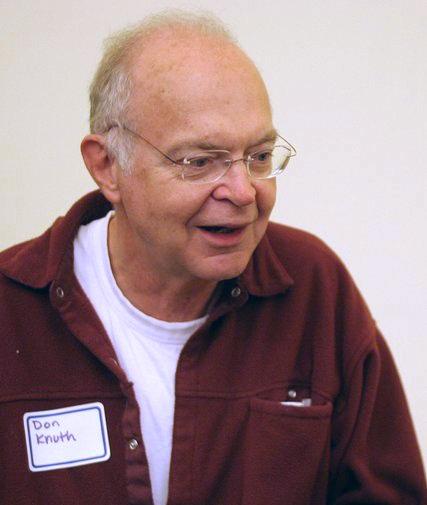
\includegraphics[width=.9\linewidth]{img/wiki-KnuthAtOpenContentAlliance.jpg}
\end{column}
\end{columns}
\end{frame}
\begin{frame}[fragile,label=sec-1-3]{Timing the code}
 \begin{block}{Prerequisites}
\begin{itemize}
\item On Windows, install biopython and cprofilev with:
\end{itemize}
\begin{verbatim}
pip install biopython
pip install cprofilev
\end{verbatim}
\begin{itemize}
\item On Mac and GNU/Linux, use:
\end{itemize}
\begin{verbatim}
sudo pip install biopython
sudo pip install cprofilev
\end{verbatim}
\end{block}
\end{frame}
\begin{frame}[label=sec-1-4]{Timing the code}
\begin{block}{Run time depends on input size}
\begin{itemize}
\item We'll make together one Python script that tests if a sequence can be DNA
\item We'll time its execution on several input files of different size
\end{itemize}
\end{block}
\begin{block}{Worst case/best case scenario}
\end{block}
\end{frame}
\begin{frame}[fragile,label=sec-1-5]{Timing the code}
 \begin{block}{Live coding}
\begin{itemize}
\item Using \texttt{BioPython} to parse fasta files
\end{itemize}
\end{block}
\end{frame}

\begin{frame}[label=sec-1-6]{Scaling}
linear dependence, exponential dependence
\end{frame}
\begin{frame}[label=sec-1-7]{Profiling}
\url{https://docs.python.org/2/library/profile.html#instant-user-s-manual}
\end{frame}
\begin{frame}[label=sec-1-8]{Bottleneck}
Is it the loading? Is it the loop?
\end{frame}
\section{Introduction to the shell}
\label{sec-2}

\begin{frame}[fragile,label=sec-2-1]{What is the shell?}
 \begin{block}{In brief\ldots{}}
\begin{itemize}
\item Command line interface, looks old-fashioned but very convenient
\item Main interface when you want to login to \alert{CSC servers} or \alert{remote servers}
\item Also present in \alert{Linux} distributions for personal computers and \alert{Mac}
\item With \alert{Windows}, the \texttt{cmd} prompt is a bit similar (text-based) but not as
powerful
\end{itemize}
\end{block}
\begin{block}{Usage}
\begin{itemize}
\item Often the only interface for remote connections
\item Powerful built-in commands
\item \alert{Automate repetitive tasks}
\item Shell scripts to \alert{reproduce} data manipulation
\end{itemize}
\end{block}
\end{frame}
\begin{frame}[fragile,label=sec-2-2]{Where can we find the shell?}
 \begin{block}{To find a shell\ldots{}}
\begin{itemize}
\item On \alert{GNU/Linux} and \alert{MacOS} systems: open a \alert{terminal}. This will provide you
with a Unix-like shell on both systems
\item On \alert{Windows}: run \texttt{cmd.exe} or \texttt{cmd}. This shell is quite different from the
Unix-like shell found in Linux and MacOS. To obtain a Unix shell on Windows,
one can install the \href{https://www.cygwin.com/}{Cygwin} tools.
\item It is strongly recommended to learn how to use a \alert{Unix shell} since it is
very likely it is this type of shell you will be exposed to when you connect
to a \alert{remote server}.
\end{itemize}
\end{block}
\end{frame}
\begin{frame}[label=sec-2-3]{Where can we find the shell?}
\begin{block}{One shell or several shells?}
\begin{itemize}
\item A shell: a program providing an \alert{interface} between the user and the
computer. \alert{Different shells exist}.
\item The most popular and widely used shell is probably \alert{bash}. It is the
default shell in most GNU/Linux distributions.
\item If you learn how to use \alert{bash}, you will be able to use most \alert{remote servers}
you'll have to connect to, and also the \alert{terminal} from MacOS or the \alert{Cygwin}
tools on Windows
\end{itemize}
\end{block}
\begin{block}{One word on terminology}
\begin{itemize}
\item During the course, we will often say interchangeably "the terminal", "the
shell" or "bash".
\end{itemize}
\end{block}
\end{frame}
\begin{frame}[label=sec-2-4]{The CSC center in Kajaani}
\begin{center}
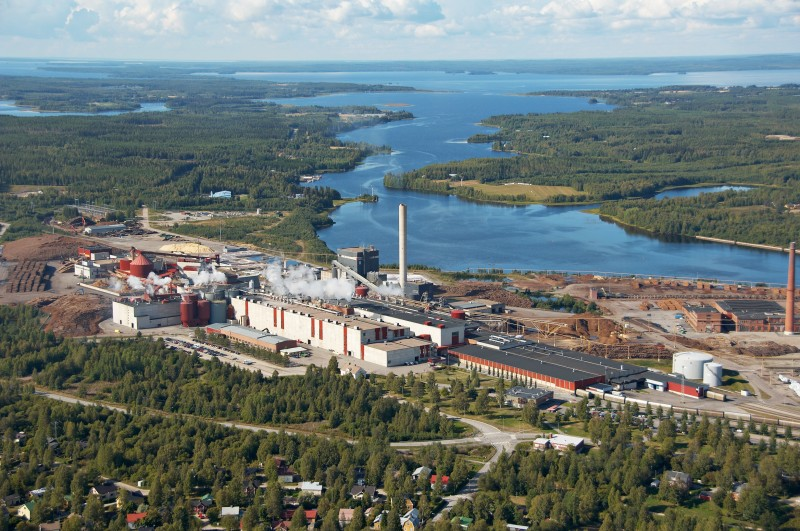
\includegraphics[width=.9\linewidth]{img/digitice-csc-kajaani-800_ilmakuva_tehtaasta.jpg}
\end{center}
\end{frame}
\begin{frame}[fragile,label=sec-2-5]{Meet the Taito cluster (\texttt{taito.csc.fi})}
 \begin{center}
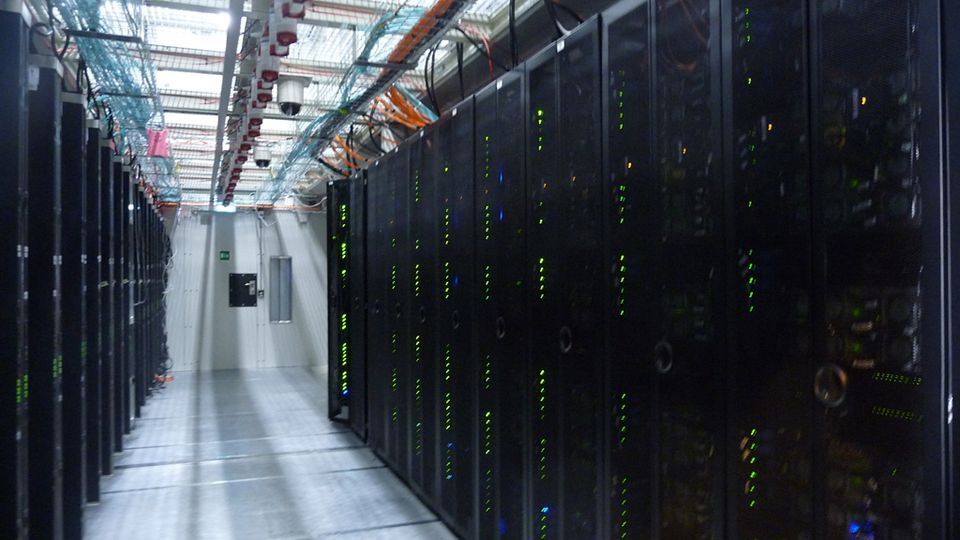
\includegraphics[width=.9\linewidth]{img/yle-taito-supertietokone-kajaani.jpg}
\end{center}
\end{frame}
\begin{frame}[label=sec-2-6]{A word about CSC servers}
\begin{block}{Available servers}
\begin{itemize}
\item Taito: 19152 cores (16 cores per nodes)
\item Sisu: 39408 cores, for massively parallel jobs
\end{itemize}
\end{block}
\begin{block}{Job submission}
\begin{itemize}
\item CPU-intense calculations have to be submitted through a queue system
\item \href{https://sui.csc.fi/group/sui/host-monitor}{Server load}
\item We can also run some simple commands directly at login
\end{itemize}
\end{block}
\begin{block}{Module system}
\begin{itemize}
\item Many softwares installed
\item Sometimes different versions of a software
\item User has to explicitly load \alert{modules}
\end{itemize}
\end{block}
\end{frame}
\begin{frame}[fragile,label=sec-2-7]{Connection to a remote shell}
 \begin{block}{The plan}
\begin{itemize}
\item Using the CSC server Taito in Kajaani (student account)
\item Tools: \alert{putty} (windows) or \alert{ssh} (Mac and GNU/Linux)
\item A word about \alert{ssh} and the \alert{security of connections}?
\end{itemize}
\end{block}
\begin{block}{Student account}
\begin{itemize}
\item Logins: \texttt{jyybio01} to \texttt{jyybio20}
\item Password: on the whiteboard
\end{itemize}
\end{block}
\begin{block}{Connection}
\begin{itemize}
\item From a terminal (Mac or GNU/Linux):
\begin{verbatim}
ssh jyybioxx@taito.csc.fi
\end{verbatim}
where \texttt{xx} is your student number.
\item From Putty: ask a teacher if needed
\end{itemize}
\end{block}
\end{frame}
\begin{frame}[fragile,label=sec-2-8]{First contact with the shell}
 \begin{block}{Just after connection}
\begin{itemize}
\item What you see after connection in the \alert{shell prompt}. It tells you the shell
is ready to receive your input:
\begin{verbatim}
jyybioxx@taito-login3$
\end{verbatim}
\item \texttt{jyybioxx} is your username, \texttt{taito-login} is the host server to which you
are connected. The number after \texttt{taito-login} can vary because Taito has
several login nodes.
\end{itemize}
\end{block}
\end{frame}
\begin{frame}[fragile,label=sec-2-9]{First contact with the shell}
 \begin{block}{Execute a command (\texttt{ls})}
The shell \alert{reads} and \alert{executes} commands you enter at the prompt, and \alert{prints}
the output. Type \texttt{ls} and press \texttt{RETURN}. You should see:
\begin{verbatim}
appl_taito
\end{verbatim}
\end{block}
\begin{block}{}
You just ran the \texttt{ls} command which produces an output: the list of files and
folders present in the current directory. 

\begin{itemize}
\item Try another command: \texttt{whoami}. What does this command do?
\end{itemize}
\end{block}
\end{frame}
\begin{frame}[fragile,label=sec-2-10]{First contact with the shell}
 \begin{block}{Execute a command (\texttt{pwd})}
\begin{itemize}
\item When you login to a server, you are automatically sent to your home
folder. You can see where you are by typing \texttt{pwd}, which produces:
\begin{verbatim}
/homeappl/home/jyybioxx
\end{verbatim}
\item So you are now in the folder \texttt{jyybioxx}, which is itself contained in \texttt{home},
which is contained in \texttt{homeappl}, which is at the root of the file system
(\texttt{/}, there is no parent directory above).
\end{itemize}
\end{block}
\end{frame}
\begin{frame}[fragile,label=sec-2-11]{Adding options to a command}
 \begin{block}{Using \texttt{ls} options}
\begin{itemize}
\item You can add options to a command with the dash sign \texttt{-}:
\begin{verbatim}
ls -l
\end{verbatim}
(this is -l, not -1)

\item This runs the \texttt{ls} command with the \texttt{-l} option, which produces a detailed
output:
\begin{verbatim}
total 4
drwx------ 2 jyybio20 jyybio 4096 Apr 15 12:15 appl_taito
\end{verbatim}
Now you can see the date of last modification of the folders and some other
information.
\end{itemize}
\end{block}
\end{frame}
\begin{frame}[fragile,label=sec-2-12]{A word about rights}
 \begin{block}{The rights system}
\begin{itemize}
\item In a Unix system, every file has an \alert{owner} and belongs to a \alert{group}
\item Every file has rights for \alert{reading}, \alert{writing} and \alert{execution}
\item Those rights are set for three categories of users: \alert{owner}, \alert{group} and
  \alert{others}
\end{itemize}
\end{block}
\begin{block}{\texttt{ls -l} output}
\texttt{drwx-{}-{}-{}-{}-{}- 2 jyybio20 jyybio 4096 Apr 15 12:15 appl\_taito}
\begin{itemize}
\item The three first letters are rights for the owner, the next three rights for
the group, and the last three rights for others.
\item If a letter is replaced by a dash, the right is not granted
\end{itemize}
\begin{verbatim}
-rwx------
-r--r--r--
-rwxr--r--
drwxr-xr-x
\end{verbatim}
\end{block}
\end{frame}
\begin{frame}[fragile,label=sec-2-13]{Clone the Git repository for the practicals}
 \begin{block}{Clone the Git repository}
\begin{itemize}
\item Before going further, you should clone a Git repository containing the data
which was prepared for you (Git is installed on Taito). The repository is
hosted on GitHub.

\item Check that you are in your home folder with \texttt{pwd}. You should see:
\begin{verbatim}
/homeappl/home/jyybioxx
\end{verbatim}
If not, go back to your home folder by typing simply \texttt{cd} without any
argument.

\item Clone the Git repository with (all on one line):
\end{itemize}
\begin{verbatim}
git clone 
https://github.com/mdjbru-teaching-material/practicals.git
\end{verbatim}

\begin{itemize}
\item Run \texttt{ls}. What happened?
\end{itemize}
\end{block}
\end{frame}
\begin{frame}[label=sec-2-14]{Data content and motivation}
\begin{block}{The data files}
\begin{itemize}
\item Each \alert{file} corresponds to \alert{one \emph{Escherichia coli} strain} for which a
complete or draft genome sequence is available. Each file contains the
\alert{peptide sequences} from all translations resulting from Ensembl known or
novel gene predictions for that strain.

\item Files are in the FASTA format. The original address is
  \url{ftp://ftp.ensemblgenomes.org/pub/current/bacteria/fasta/}.
\end{itemize}
\end{block}
\begin{block}{Motivation}
We want to determine the \alert{amino acid content} of \alert{all proteins of each strain},
and compare the results between strains. We already have a Python script ready
which can determine the amino-acid composition for protein sequences.
\end{block}
\end{frame}
\begin{frame}[fragile,label=sec-2-15]{Basic folder navigation}
 \begin{block}{\texttt{cd} command}
\begin{itemize}
\item We can navigate from folder to folder using the \texttt{cd} command:
\end{itemize}
\begin{verbatim}
cd practicals
ls
cd ecoli-data
ls
\end{verbatim}
\begin{itemize}
\item We could have gone directly to the second subfolder with:
\end{itemize}
\begin{verbatim}
cd practicals/ecoli-data
\end{verbatim}

\begin{itemize}
\item You can see there are already some files in this folder. Let's ask for more
details with \texttt{ls -l}

\item How many files are there? How large are they?
\end{itemize}
\end{block}
\end{frame}
\begin{frame}[fragile,label=sec-2-16]{Basic folder navigation}
 \begin{block}{Combining options for \texttt{ls}}
\begin{itemize}
\item We can ask for more human-readable sizes with:
\end{itemize}
\begin{verbatim}
ls -l -h
\end{verbatim}
\begin{itemize}
\item Can you see the difference with \texttt{ls -l}? What does \texttt{ls -h} do?
\item We could also combine both options to \texttt{ls}: \texttt{ls -lh}
\end{itemize}
\end{block}
\end{frame}
\begin{frame}[fragile,label=sec-2-17]{Basic folder navigation}
 \begin{block}{Moving to the parent directory}
\begin{itemize}
\item We can go back through the parent folders using \texttt{cd ..}
\end{itemize}
\begin{verbatim}
pwd    # Where are you at this point?
cd ..
pwd    # And now?
ls
cd ..
pwd    # And here?
ls
\end{verbatim}
\end{block}
\end{frame}
\begin{frame}[fragile,label=sec-2-18]{Basic folder navigation}
 \begin{block}{Going back to the home directory}
\begin{itemize}
\item A faster way to go back to your home directory, from any starting directory,
is just to type \texttt{cd} without any argument.
\item Go back to the \texttt{ecoli-data} subfolder and back again to your home directory
using \texttt{cd}.
\end{itemize}
\end{block}
\begin{block}{Shortcut for the home folder}
\begin{itemize}
\item Another way to go to the home folder is to use the \texttt{\textasciitilde{}} character: this is
automatically replaced by the path to your home folder by \texttt{bash}.
\end{itemize}
\begin{verbatim}
cd     # Back to your home folder
cd practicals
cd ~   # Bash understands "~" as "/homeappl/home/jyybioxx"
cd appl_taito
cd ~/practicals
\end{verbatim}
\end{block}
\end{frame}
\begin{frame}[fragile,label=sec-2-19]{Creating folders}
 \begin{block}{The \texttt{mkdir} command}
\begin{itemize}
\item Go back to the \texttt{practicals} folder and create a new folder in it:
\end{itemize}
\begin{verbatim}
cd ~/practicals
mkdir results
cd results
ls
\end{verbatim}
\end{block}
\begin{block}{Exercise}
\begin{itemize}
\item Create the following directory structure:
\end{itemize}
\begin{verbatim}
~/practicals/scripts/python/modules/seqAnalysis
\end{verbatim}
\begin{itemize}
\item Go back to your home folder.
\end{itemize}
\end{block}
\end{frame}
\begin{frame}[fragile,label=sec-2-20]{Auto-completion}
 \begin{block}{The magic \texttt{TAB} key}
\begin{itemize}
\item Let's go into \texttt{seqAnalysis} folder, but let's be lazy:
\end{itemize}
\begin{verbatim}
cd     # Start from your home folder
cd pr  # Press TAB at this point
\end{verbatim}
\begin{itemize}
\item Do you understand what happened?
\item Use this feature to quickly go to \texttt{seqAnalysis}. What is the minimum number
of keystrokes you have to use to go there from your home folder?
\end{itemize}
\end{block}
\begin{block}{Remember!}
When you press \alert{\texttt{TAB}}, the shell tries to complete what you just typed by
itself. This \alert{auto-completion feature} of the shell is very convenient and will
save you a lot of typing!
\end{block}
\end{frame}
\begin{frame}[fragile,label=sec-2-21]{Auto-completion}
 \begin{block}{Test auto-completion}
\begin{itemize}
\item Now create a folder:
\end{itemize}
\begin{verbatim}
~/practicals/scripts/python/modifiedSources
\end{verbatim}
\begin{itemize}
\item Go back to your home folder, and go into \texttt{modifiedSources} using the \texttt{TAB}
completion as much as you can. What do you notice?
\end{itemize}
\end{block}
\end{frame}
\begin{frame}[fragile,label=sec-2-22]{Auto-completion}
 \begin{block}{Double \texttt{TAB}}
\begin{itemize}
\item Now create the folder
\end{itemize}
\begin{verbatim}
~/practicals/scripts/python/modularComponents
\end{verbatim}
\begin{itemize}
\item Type:
\end{itemize}
\begin{verbatim}
cd ~/practicals/scripts/python/mod # Press =TAB= twice here
# Type "ule" and press =TAB= again
\end{verbatim}
\begin{itemize}
\item Do you understand how \texttt{TAB} completion works? This also works for command
names.
\end{itemize}
\end{block}
\end{frame}
\begin{frame}[fragile,label=sec-2-23]{Copying, moving and removing files}
 \begin{block}{Creating an empty file}
\begin{itemize}
\item Go the the \texttt{seqAnalysis} folder and type:
\end{itemize}
\begin{verbatim}
touch DNA-analysis.py
ls
\end{verbatim}
\begin{itemize}
\item What happened?
\end{itemize}
\end{block}
\begin{block}{Moving a file}
\begin{itemize}
\item Now type:
\end{itemize}
\begin{verbatim}
mv DNA-analysis.py ../modularComponents
\end{verbatim}
\begin{itemize}
\item What happened? Did you use the \texttt{TAB} key? (you should!)
\item Explore the directory structure to find \texttt{DNA-analysis.py} again.
\end{itemize}
\end{block}
\end{frame}
\begin{frame}[fragile,label=sec-2-24]{Copying, moving and removing files}
 \begin{block}{Copying a file}
\begin{itemize}
\item Go to the \texttt{modularComponents} subfolder and type:
\end{itemize}
\begin{verbatim}
cp DNA-analysis.py ../modules
\end{verbatim}
\begin{itemize}
\item What happened?
\end{itemize}
\end{block}
\begin{block}{Removing a file}
\begin{itemize}
\item From \texttt{modularComponents} folder, type:
\end{itemize}
\begin{verbatim}
rm DNA-analysis.py
\end{verbatim}
\begin{itemize}
\item What happened?
\end{itemize}
\end{block}
\end{frame}
\begin{frame}[fragile,label=sec-2-25]{Creating a directory hierarchy}
 \begin{block}{Moving a folder}
\begin{itemize}
\item From the \texttt{scripts} folder, move \texttt{modularComponents} into \texttt{modules}:
\end{itemize}
\begin{verbatim}
mv modularComponents modules
tree
\end{verbatim}
\begin{itemize}
\item What does \texttt{tree} do?
\end{itemize}
\end{block}
\begin{block}{Copying a folder}
\begin{itemize}
\item Go to the \texttt{practicals} folder and make a copy of \texttt{scripts}:
\end{itemize}
\begin{verbatim}
cp -r scripts scripts-backup
\end{verbatim}
\begin{itemize}
\item Note the \texttt{-r} option used for recursive copy inside the directories.
\end{itemize}
\end{block}
\end{frame}
\begin{frame}[fragile,label=sec-2-26]{Creating a directory hierarchy}
 \begin{block}{Removing a folder}
\begin{itemize}
\item Remove the newly created folder with:
\end{itemize}
\begin{verbatim}
rm -r scripts-backup
\end{verbatim}
\begin{itemize}
\item Again, note the \texttt{-r} option to work on folders.
\end{itemize}
\end{block}
\end{frame}
\begin{frame}[fragile,label=sec-2-27]{Creating a directory hierarchy}
 \begin{block}{Exercise}
\begin{itemize}
\item Now that you have experience, create the exact following directory structure
(only folders shown):
\end{itemize}
\begin{verbatim}
+-- appl_taito
`-- practicals
    +-- ecoli-data
    |   `-- [...]
    +-- results
    |   `-- 2015-04-22
    `-- scripts
        +-- python
        |   +-- popGenetics
        |   +-- proteinStructure
        |   `-- seqAnalysis
        `-- R
\end{verbatim}
\end{block}
\end{frame}
\begin{frame}[fragile,label=sec-2-28]{Viewing a file}
 \begin{block}{\texttt{cat} command}
\begin{itemize}
\item Go to the \texttt{ecoli-data} folder and type:
\end{itemize}
\begin{verbatim}
cat README
\end{verbatim}
\begin{itemize}
\item Try also \texttt{cat} on one of the fasta files. What happened?
\end{itemize}
\end{block}
\begin{block}{\texttt{head} and \texttt{tail} commands}
\begin{verbatim}
head Escherichia_coli_o5_k4_l_h4_str_atcc_23502.GCA_000333195.1.26.pep.all.fa
tail Escherichia_coli_o5_k4_l_h4_str_atcc_23502.GCA_000333195.1.26.pep.all.fa
head -n 30 Escherichia_coli_o5_k4_l_h4_str_atcc_23502.GCA_000333195.1.26.pep.all.fa
tail -n 3 Escherichia_coli_o5_k4_l_h4_str_atcc_23502.GCA_000333195.1.26.pep.all.fa
\end{verbatim}
\begin{itemize}
\item Do you understand what those commands do?
\end{itemize}
\end{block}
\end{frame}
\begin{frame}[fragile,label=sec-2-29]{Viewing a file}
 \begin{block}{\texttt{less} command}
\begin{itemize}
\item \texttt{less} is very useful to examine large file. You can navigate using the up
and down arrows or \texttt{B} and \texttt{SPACE} keys, and you can exit with \texttt{Q}.
\end{itemize}
\begin{verbatim}
less Escherichia_coli_o5_k4_l_h4_str_atcc_23502.GCA_000333195.1.26.pep.all.fa
\end{verbatim}
\end{block}
\end{frame}
\section{Shell tools}
\label{sec-3}

\begin{frame}[fragile,label=sec-3-1]{Useful tools: \texttt{wc}}
 \begin{block}{\texttt{wc} to count words}
\begin{itemize}
\item Go to the \texttt{ecoli-data} folder and type:
\end{itemize}
\begin{verbatim}
wc Escherichia_coli_o55_h7_str_06_3555.GCA_000617385.1.26.pep.all.fa
\end{verbatim}
which produces:
\begin{verbatim}
26318   51865 1824223 Esch...
\end{verbatim}
\begin{itemize}
\item We can have only the number of lines with \texttt{wc -l} (try it).
\end{itemize}
\end{block}
\begin{block}{Wildcards}
\begin{itemize}
\item Try:
\end{itemize}
\begin{verbatim}
wc -l *.fa
\end{verbatim}
\begin{itemize}
\item What happened?
\end{itemize}
\end{block}
\end{frame}
\begin{frame}[fragile,label=sec-3-2]{Redirection}
 \begin{block}{The \texttt{>} operator}
\begin{itemize}
\item When a command produces some output, it can be redirected to a file instead
of to the terminal:
\end{itemize}
\begin{verbatim}
wc -l *.fa > lineCounts
cat lineCounts
\end{verbatim}
\begin{itemize}
\item \texttt{>} is a \alert{redirection} operator, and automatically creates a new file or
erases an existing file.
\end{itemize}
\end{block}
\begin{block}{The \texttt{>>} operator}
\begin{itemize}
\item To redirect output and append it to an existing file, we can use the \texttt{>>}
operator:
\end{itemize}
\begin{verbatim}
wc -l README >> lineCounts
cat lineCounts
\end{verbatim}
\end{block}
\end{frame}
\begin{frame}[fragile,label=sec-3-3]{Useful tools: \texttt{grep}}
 \begin{block}{\texttt{grep} to search for matches}
\begin{verbatim}
grep "flagellin" Escherichia_coli_o55_h7_str_06_3555.GCA_000617385.1.26.pep.all.fa
grep --color=always "flagellin" Escherichia_coli_o55_h7_str_06_3555.GCA_000617385.1.26.pep.all.fa
grep -n --color=always "flagellin" Escherichia_coli_o55_h7_str_06_3555.GCA_000617385.1.26.pep.all.fa
grep -c --color=always "flagellin" Escherichia_coli_o55_h7_str_06_3555.GCA_000617385.1.26.pep.all.fa
\end{verbatim}
\begin{itemize}
\item Do you understand what each of the \texttt{grep} options do?
\end{itemize}
\end{block}
\begin{block}{Exercise}
\begin{itemize}
\item Use \texttt{grep} to extract all the sequence names from one of the fasta file and
store them in a file called \texttt{proteinNames}.
\end{itemize}
\end{block}
\end{frame}
\begin{frame}[fragile,label=sec-3-4]{Useful tools: \texttt{grep}}
 \begin{block}{\texttt{grep} is versatile}
\begin{verbatim}
grep -c flagellin *.fa
grep -c flagel *.fa
\end{verbatim}
\begin{itemize}
\item Do you understand the output?
\end{itemize}
\end{block}
\begin{block}{Exercise}
\begin{itemize}
\item How would you count the number of proteins in each fasta file?
\end{itemize}
\end{block}
\end{frame}
\begin{frame}[fragile,label=sec-3-5]{Useful tools: \texttt{cut}}
 \begin{block}{\texttt{cut} to get columns}
\begin{verbatim}
grep -c flagel *.fa > flagelCounts
cat flagelCounts
cut -d "_" -f 1 flagelCounts
cut -d "_" -f 3 flagelCounts
cut -d "_" -f 3,5 flagelCounts
cut -d ":" -f 2 flagelCounts
\end{verbatim}
\begin{itemize}
\item Do you understand what \texttt{cut} does and the roles of the \texttt{-d} and \texttt{-f} options?
\end{itemize}
\end{block}
\end{frame}
\begin{frame}[fragile,label=sec-3-6]{Useful tools: \texttt{sort}}
 \begin{block}{\texttt{sort} to sort things}
\begin{itemize}
\item Use \texttt{sort} to sort the line counts from \texttt{lineCounts}:
\end{itemize}
\begin{verbatim}
sort lineCounts
\end{verbatim}
\begin{itemize}
\item Is everything correct? What if you try \texttt{sort -n lineCounts}? Can you see a
difference?
\item Try also \texttt{sort -r lineCounts}. What is the difference?
\end{itemize}
\end{block}
\begin{block}{Exercise}
\begin{itemize}
\item Using \texttt{grep} and \texttt{sort} and an intermediate files, sort the bacterial
proteomes by decreasing number of proteins.
\item Hint: \texttt{sort} supports two interesting options, \alert{\texttt{-t}} to specify a field
separator and \alert{\texttt{-k}} to specify which field to use for sorting.
\end{itemize}
\end{block}
\end{frame}
\begin{frame}[fragile,label=sec-3-7]{Combining tools with pipes}
 \begin{block}{Pipes can connect an output and an input streams}
\begin{itemize}
\item When we did \texttt{sort lineCounts}, we used \texttt{sort} on the output of \texttt{wc}, but we
used an intermediate file. The shell offers a powerful way to connect
directly the output of a command to the input of another: the \alert{pipe
operator}:
\end{itemize}
\begin{verbatim}
wc -l *.fa | sort -n
\end{verbatim}
\end{block}
\begin{block}{Exercises}
\begin{itemize}
\item The \texttt{w} output the list of connected users on the server. Try it and then
try:
\end{itemize}
\begin{verbatim}
w | head
w | less
\end{verbatim}
\begin{itemize}
\item Use a pipe to find all the users whose login contains "jyy".
\item Extend the same pipe to count how many there are.
\end{itemize}
\end{block}
\end{frame}
\begin{frame}[fragile,label=sec-3-8]{Python script to determine amino acid composition}
 \begin{block}{Test the Python script}
\begin{itemize}
\item The script \texttt{seqComposition.py} takes a fasta file and produces a table
containing the amino-acid composition of each protein in the file.
\item To run the script, type:
\end{itemize}
\begin{verbatim}
module load python-env/3.4.1   
# This module loading step is specific to the server
python3 seqComposition.py myFastaFile 
# Use the fasta file you wish instead of "myFastaFile"
\end{verbatim}
The output is sent to the terminal.
\begin{itemize}
\item Propose at least two practical ways to have a look at this output.
\end{itemize}
\end{block}
\end{frame}
\begin{frame}[label=sec-3-9]{Python script to determine amino acid composition}
\begin{block}{Exercise}
\begin{itemize}
\item Using only the \alert{Unix tools} you know, the \alert{Python script} and \alert{pipes},
determine the distribution of the number of histidines per protein in the
proteome of the strain of your choice.
\item More clearly stated: for a given strain, determines how many proteins have
one histidine, how many have two, how many have three, \ldots{}
\end{itemize}
\end{block}
\end{frame}
\section{Automating tasks}
\label{sec-4}

\begin{frame}[fragile,label=sec-4-1]{One step towards wizardry: shell scripts}
 \begin{block}{Reusing your tool pipeline}
\begin{itemize}
\item Let's use \texttt{nano} to store your pipeline in a file:
\end{itemize}
\begin{verbatim}
nano getHistDistrib.sh
\end{verbatim}
(the usage of \texttt{nano} will be demonstrated live) 
\begin{itemize}
\item The idea is to be able to produce the histidine distribution results just by
typing:
\end{itemize}
\begin{verbatim}
bash getHistDistrib.sh myFastaFile
\end{verbatim}
\end{block}
\begin{block}{Test your pipeline with a few files}
\begin{itemize}
\item Test your pipeline for 5 strains. How would you feel about doing it for 2000
strains?
\end{itemize}
\end{block}
\end{frame}
\begin{frame}[fragile,label=sec-4-2]{One step towards wizardry: shell scripts}
 \begin{block}{Making a general purpose listing script}
\begin{itemize}
\item Create a shell script (\texttt{testListing.sh}) with this content:
\end{itemize}
\begin{verbatim}
listFiles=`ls *.fa`
echo $listFiles
for myFile in $listFiles; do
    echo $myFile
    echo $myFile.results
done
\end{verbatim}
\begin{itemize}
\item Run it with \texttt{bash}. What does this do?
\end{itemize}
\end{block}
\begin{block}{Exercise: final script}
\begin{itemize}
\item Combine the script with your pipeline and the listing script into a single
script to get the histidine distribution for all the fasta files in this
folder.
\end{itemize}
\end{block}
\end{frame}
% Emacs 24.3.50.1 (Org mode 8.2.3a)
\end{document}
